\documentclass[12pt, a4paper]{article}

\usepackage{amsmath}
\usepackage{array}
\usepackage{amsmath}
\usepackage[portuguese]{babel}
\usepackage{chngpage}
\usepackage{float}
\usepackage[a4paper, margin=2cm]{geometry}
\usepackage{graphicx}
\usepackage{hyperref}
\usepackage{listings}
\usepackage{setspace}
\usepackage{xcolor}

\lstdefinestyle{codestyle}{
    language=c++,
    commentstyle=\color{teal},
    keywordstyle=\color{blue},
    numberstyle=\ttfamily\color{gray},
    stringstyle=\color{red},
    basicstyle=\ttfamily\footnotesize,
    breakatwhitespace=false,
    breaklines=false,
    keepspaces=true,
    numbers=none,
    showspaces=false,
    showstringspaces=false,
    showtabs=false,
    tabsize=4
}
\lstset{style=codestyle}

\title{\Huge \textbf{Computação Gráfica \\ \Large Trabalho Prático -- Fase I}}
\date{2 de março 2025}
\author{Grupo 3}

\begin{document}

\begin{center}
    
\includegraphics[width=0.25\textwidth]{res/cover/EE-C.eps}
\end{center}

\chardef\_=`_
\onehalfspacing
\setlength{\parskip}{\baselineskip}
\setlength{\parindent}{0pt}
\def\arraystretch{1.5}

{\let\newpage\relax\maketitle}
\maketitle
\thispagestyle{empty}

\vspace*{\fill}

\begin{adjustwidth}{-2cm}{-2cm} % These values only need to be large enough to center the table
    \begin{center}
        \begin{tabular}{>{\centering}p{0.25\textwidth}
                        >{\centering}p{0.25\textwidth}
                        >{\centering}p{0.25\textwidth}
                        >{\centering\arraybackslash}p{0.25\textwidth}}
            
\includegraphics[width=3.5cm]{res/cover/A104437.png} &
            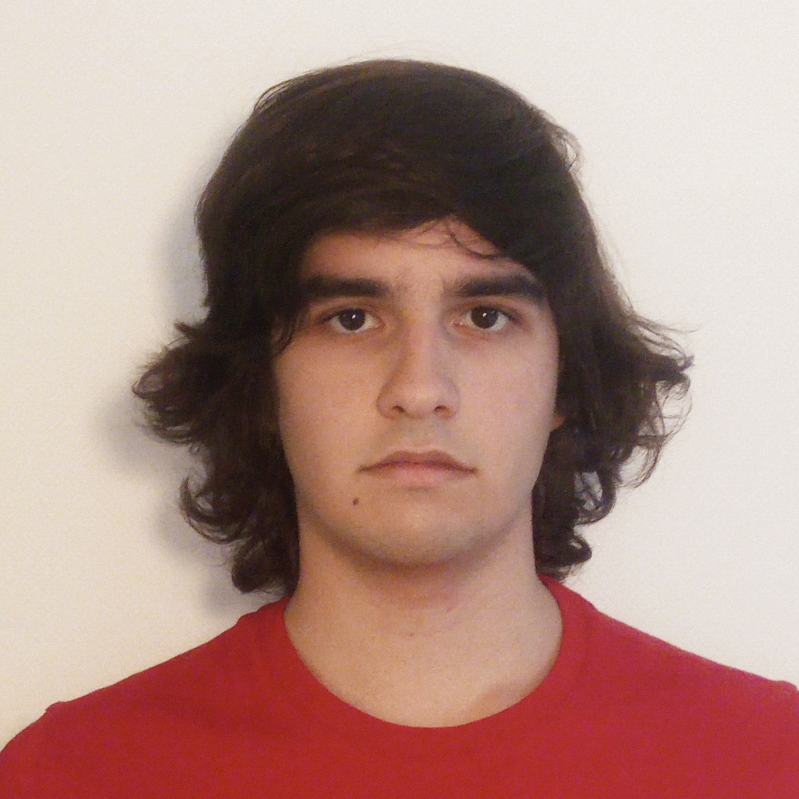
\includegraphics[width=3.5cm]{res/cover/A104348.png} &
            
\includegraphics[width=3.5cm]{res/cover/A90817.png} &
            
\includegraphics[width=3.5cm]{res/cover/A104179.png} \\

            Ana Oliveira & Humberto Gomes & Mariana Cristino & Sara Lopes \\
            A104437      & A104348        & A90817           & A104179
        \end{tabular}
    \end{center}
\end{adjustwidth}

\pagebreak

\begin{abstract}
    \textbf{\color{red} TODO - resumo}
\end{abstract}

\section{\emph{Generator}}

\subsection{Funcionamento do programa}

O programa \texttt{generator} é responsável por gerar modelos 3D de figuras geométricas, ou seja,
ficheiros com os vértices e as faces triangulares destas figuras. Nesta fase, o \texttt{generator}
deve ser capaz de gerar as seguintes figuras: planos, cubos, esferas e cones. Além de implementarmos
a geração destas figuras, como funcionalidade adicional, também desenvolvemos um gerador de
cilindros e de tori. As várias possibilidades de uso do comando \texttt{generator} são enumeradas
abaixo:

\begin{verbatim}
./generator plane    <length>      <divisions>                     <file>
./generator box      <length>      <grid>                          <file>
./generator sphere   <radius>      <slices>      <stacks>          <file>
./generator cone     <radius>      <height>      <slices> <stacks> <file>
./generator cylinder <radius>      <height>      <slices> <stacks> <file>
./generator torus    <majorRadius> <minorRadius> <slices> <stacks> <file>
\end{verbatim}

Internamente, o \texttt{generator} começa por interpretar os argumentos dados, saindo com a mensagem
acima em caso de erro. Caso contrário, gera, em memória, os conjuntos de vértices e de faces que
constituem o modelo 3D que, por fim, são escritos para um ficheiro no formato descrito abaixo.

\subsection{Formato \texttt{.3d}}

Decidimos que o formato de saída do \texttt{generator} seria o Wavefront OBJ \cite{wavefront-obj}.
O uso de um formato já existente apresentou diversas vantagens:

\begin{itemize}
    \item Foi possível desenvolver a \texttt{engine} e o \texttt{generator} em paralelo: os
        desenvolvedores do \texttt{generator} não precisavam de ter a \texttt{engine} funcional para
        testar o seu código, visto que já existem diversas ferramentas para visualizar os ficheiros
        OBJ exportados pelo \texttt{generator}.

    \item Foi possível, sem qualquer código adicional, apresentar na \texttt{engine} modelos 3D
        oriundos de ferramentas de modelação, muito mais complexos do que os gerados pelo
        \texttt{generator}.

    \item A forma de representação de faces triangulares neste formato é facilmente mapeável para
        \emph{index buffers} do OpenGL. Deste modo, não seriam necessárias alterações ao
        \texttt{generator} quando estes fossem implementados (algo que já foi feito nesta fase do
        trabalho).
\end{itemize}

O \emph{parser} desenvolvido para este formato suporta apenas o essencial para o funcionamento desta
primeira fase: posições de vértices e constituições de faces triangulares. O formato OBJ é textual,
e representar um vértice é tão simples como ter uma linha começada por um \texttt{v}, ao qual se
seguem as coordenadas do vértice separadas por espaços. O exemplo abaixo representa as coordenadas
$(0, 0.5, 1)$:

\begin{verbatim}
v 0 0.5 1
\end{verbatim}

Faces triangulares são representadas em linhas começadas por um \texttt{f}, ao qual se seguem os
índices dos três vértices da face. É de notar que a contagem dos índices começa em 1, e não em 0.
Por exemplo, para representar uma face triangular, formada pelo primeiro, segundo e terceiro
vértices do ficheiro, tem-se:

\begin{verbatim}
f 1 2 3
\end{verbatim}

Visto que a estrutura de um ficheiro \texttt{.3d} separa os vértices de um modelo das suas faces, o
processo de criação dos modelos 3D dos vários sólidos é dividido em duas fases: a geração do
conjunto de pontos que os constituem, e o seu agrupamento em faces triangulares.

\subsection{Plano}

O primeiro passo para a geração da nuvem de pontos de um plano é o cálculo do comprimento de uma
divisão, $d = \frac{L}{N}$, onde $L$ simboliza o comprimento do plano e $N$ o número de divisões.
Depois, determinam-se os dois vetores que definem a direção do plano. Estes poderiam ser os vetores
diretores dos eixos $x$ e $z$, mas é mais simples que estes tenham o comprimento de uma divisão do
plano.

$$
\vec{\imath} = (d, 0, 0)
\hspace{1cm}
\vec{\jmath} = (0, 0, d)
$$

Depois, encontra-se o ponto do plano com os menores valores das coordenadas $x$ e $z$. Como se
deseja que o plano esteja centrado na origem, as coordenadas $x$ e $z$ do ponto desejado serão o
simétrico da metade do comprimento do plano:

$$
P_0 = \left ( - \frac{L}{2}, 0, - \frac{L}{2} \right )
$$

Depois, qualquer ponto $P$ do plano pode ser definido como a adição a $P_0$ de uma combinação linear
de $\vec{\imath}$ e $\vec{\jmath}$, limitando a números inteiros os coeficientes multiplicativos dos
vetores:

$$
P = P_0 + \alpha \, \vec{\imath} + \beta \, \vec{\jmath}
\hspace{1cm}
\alpha, \beta \in \left \lbrace 0, 1, \ldots, N \right \rbrace
$$

Na prática, o plano é gerado iterando pelos valores inteiros possíveis de $\alpha$ e de $\beta$,
incrementando primeiro $\beta$, e só depois de $\alpha$, o que dá origem a uma nuvem de pontos como
a que pode ser observada na figura abaixo:

\begin{figure}[H]
    \centering
    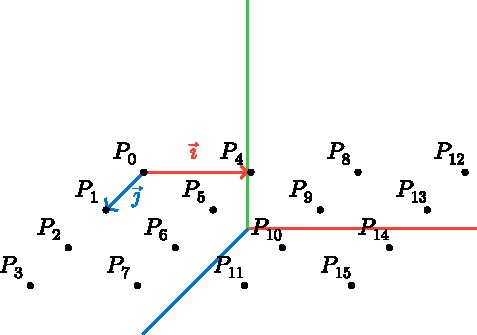
\includegraphics[width=0.4\textwidth]{res/figures/PlanePoints.pdf}
    \caption{Nuvem de pontos resultante da geração de um plano de três divisões.}
\end{figure}

Depois, os vértices gerados podem ser agrupados nos triângulos que formam o plano. Para tal,
começa-se com o primeiro vértice do plano, $P_0$. Considera-se também o vértice seguinte, $P_1$, e
os dois vértices com os valores de $z$ de $P_0$ e $P_1$, mas com o seguinte valor de $x$ possível
(na "linha"{} seguinte). Um exemplo de um conjunto destes quatro vértices pode ser visto na figura
abaixo. Com estes vértices, gera-se um quadrado, ou seja, dois triângulos. Este processo repete-se
para todos os vértices onde é aplicável, ou seja, todos com exceção dos pontos com os maiores
valores de $x$ ou de $z$ possíveis.

\begin{figure}[H]
    \centering
    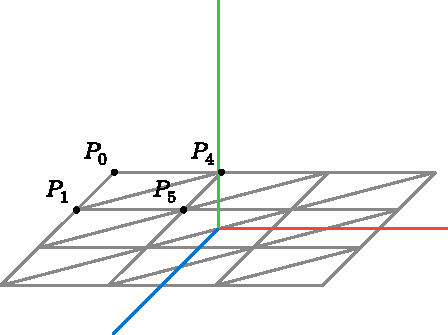
\includegraphics[width=0.4\textwidth]{res/figures/PlaneTriangles.pdf}
    \caption{
        Triângulos de um plano gerado, e pontos utilizados na primeira iteração do ciclo de geração
        de triângulos.
    }
\end{figure}

Uma otimização feita pela \emph{engine} é \emph{face culling}, ou seja, desenhar apenas as faces
voltadas para a câmara. No caso do plano, deseja-se que os seus triângulos estejam voltados para
cima, pelo que os seus vértices devem estar ordenados na ordem contrária à dos ponteiros do
relógio. Para os quatro pontos apresentados acima, os triângulos gerados são os seguintes:

$$
T_1 = (P_1, P_4, P_0)
\hspace{1cm}
T_2 = (P_1, P_5, P_4)
$$

\subsection{Cubo}

De um modo simples, o processo de geração de um cubo consiste na repetição da geração de um plano
seis vezes, uma vez para cada face. No entanto, algumas diferenças devem ser evidenciadas. Tal como
no plano, após ser calculado o comprimento de uma divisão do cubo, são definidos os vetores
diretores dos vários planos que são as faces do cubo. Há três pares de vetores diretores, cada um
utilizado para gerar duas faces opostas:

$$
\begin{array}{ll>{\hspace{1cm}}ll>{\hspace{1cm}}c}
    \vec{\imath_1} &= (1, 0, 0) &
    \vec{\jmath_1} &= (0, 1, 0) &
    (\text{faces dianteira e traseira}) \\
    \vec{\imath_2} &= (0, 1, 0) &
    \vec{\jmath_2} &= (0, 0, 1) &
    (\text{faces esquerda e direita}) \\
    \vec{\imath_3} &= (0, 0, 1) &
    \vec{\jmath_3} &= (1, 0, 0) &
    (\text{faces superior e inferior})
\end{array}
$$

Ao contrário do que acontece no plano, estes vetores encontram-se normalizados, o que é útil para
determinar o ponto de cada face a partir do qual os seus restantes pontos serão gerados. Tal como
acontece no plano, para o cubo estar centrado na origem, é necessário que todas as coordenadas deste
ponto inicial estejam a uma distância de $\frac{L}{2}$ da origem, onde $L$ representa o comprimento
do lado do cubo. Por exemplo, para o primeiro par de vetores diretores, os pontos são os seguintes,
correspondentes às faces traseira e dianteira, respetivamente:

$$
P_{0^-} = \left ( -\frac{L}{2}, -\frac{L}{2}, -\frac{L}{2} \right )
\hspace{1cm}
P_{0^+} = \left ( -\frac{L}{2}, -\frac{L}{2}, +\frac{L}{2} \right )
$$

De um modo geral, nas coordenadas onde $\vec{\imath}$ ou $\vec{\jmath}$ têm um valor não nulo, a
coordenada do ponto inicial é $-\frac{L}{2}$. A coordenada restante pode assumir, conforme a face,
ou $\frac{L}{2}$ ou $-\frac{L}{2}$. Matematicamente, o vetor perpendicular à face é dado por:

$$
\vec{n} = (1, 1, 1) - \vec{\imath} - \vec{\jmath}
$$

A partir deste vetor, os pontos iniciais das faces são dados por:

$$
P_{0^-} = -\frac{L}{2} \left ( \vec{\imath} + \vec{\jmath} + \vec{n} \right )
\hspace{1cm}
P_{0^+} = -\frac{L}{2} \left ( \vec{\imath} + \vec{\jmath} - \vec{n} \right )
$$

Com os vetores diretores e os pontos iniciais de cada face, é possível normalizar os vetores
diretores e gerar os pontos de cada face, seguindo o mesmo processo utilizado para o plano. Abaixo,
apresenta-se um exemplo da nuvem de pontos de um cubo gerado:

\begin{figure}[H]
    \centering
    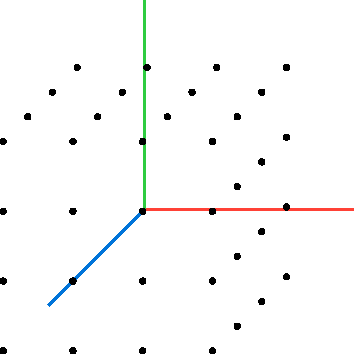
\includegraphics[width=0.35\textwidth]{res/figures/CubePoints.pdf}
    \caption{
        \onehalfspacing
        Nuvem de pontos resultante da geração de um cubo de três divisões. Os pontos das faces
        ocultas não foram representados nesta figura.
    }
\end{figure}

Depois de gerada a nuvem de pontos, o processo de geração dos triângulos de cada face é muito
semelhante ao do plano. No entanto, a ordem dos vértices de cada triângulo difere conforme a face do
cubo a ser construída. Considere-se o exemplo abaixo, o das faces superior e inferior de um cubo com
apenas uma divisão:

\begin{figure}[H]
    \centering
    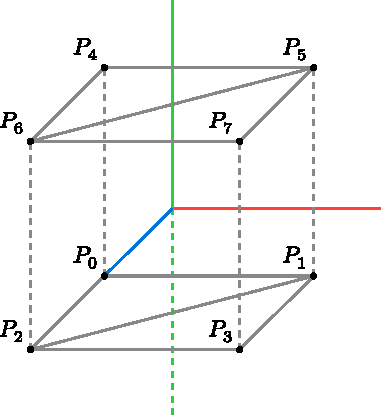
\includegraphics[width=0.35\textwidth]{res/figures/CubeFaces.pdf}
    \caption{Faces superior e inferior de um cubo de apenas uma divisão.}
\end{figure}

Para que os triângulos da face inferior estejam voltados para o exterior do cubo, ou seja, para
baixo, os seus pontos são ordenados no sentido dos ponteiros do relógio:

$$
T_1 = (P_1, P_2, P_0)
\hspace{1cm}
T_2 = (P_1, P_3, P_2)
$$

Na face superior, a ordem dos pontos dos triângulos é contrária, no sentido contrário ao dos
ponteiros do relógio:

$$
T_1' = (P_5, P_4, P_6)
\hspace{1cm}
T_2' = (P_7, P_5, P_6)
$$

Para cada par de faces opostas, cada face será sujeita, conforme o seu vetor normal, a uma ordenação
distinta dos pontos dos seus triângulos. Após aplicar o processo de geração de triângulos a todas as
faces, é dada por concluída a construção do modelo do cubo.

\begin{figure}[H]
    \centering
    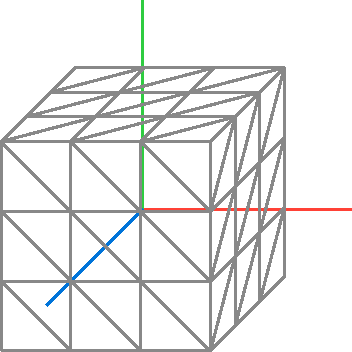
\includegraphics[width=0.35\textwidth]{res/figures/CubeTriangles.pdf}
    \caption{
        \onehalfspacing
        Triângulos resultantes da geração de um cubo de três divisões. As faces ocultas não foram
        representadas nesta figura.
    }
\end{figure}

\subsection{Esfera}

Para a construção da esfera, utilizámos um sistema de coordenadas esféricas,
no qual a posição de cada ponto na esfera é determinada por dois ângulos: o
ângulo polar \( \theta \) e o ângulo azimutal \( \phi \).

A parametrização de um ponto sobre uma esfera de raio \( r \) pode ser definida pelas seguintes
equações:
\[
x = r \sin(\theta) \cos(\phi)
\]
\[
y = r \cos(\theta)
\]
\[
z = r \sin(\theta) \sin(\phi)
\]
onde:
\begin{itemize}
\item \( \theta \) é o ângulo polar, que varia entre \( 0 \) (pólo norte) e \( \pi \)
(pólo sul), que determina a latitude do ponto na esfera;
\item \( \phi \) é o ângulo azimutal que varia entre \( 0 \) e \( 2\pi \), que define a
longitude do ponto.
\end{itemize}

Este modelo matemático permite gerar uma esfera distribuída no espaço tridimensional.
No entanto, para a sua implementação computacional, é necessário discretizar estes valores e
definir um conjunto finito de pontos e faces que aproximem à sua forma contínua.

\subsubsection{Geração dos Vértices}
Para discretizar a superfície da esfera, divide-se o intervalo de \( \theta \) em stacks
(fatias horizontais) e o intervalo de \( \phi \) em slices (segmentos verticais). Assim,
as incrementações angulares são calculados da seguinte forma:
\[
\Delta\theta = \frac{\pi}{\text{stacks}}, \quad \Delta\phi = \frac{2\pi}{\text{slices}}
\]
Ao percorrer os valores de \( \theta \) e \( \phi \), é possível gerar um conjunto ordenado
de pontos distribuídos sobre a esfera.

De modo que, a construção dos vértices segue os seguintes passos:

1. Criação do pólo norte: O primeiro ponto criado é o pólo norte, localizado em
\( (0, r, 0) \).

2. Geração dos Pontos Intermédios: Para cada stack (exceto as extremidades, que
são os pólos), iterámos sobre os valores de \( \theta \), determinámos a altura \( y \) do ponto
e o raio da secção circular correspondente:
\[
y = r \cos(\theta)
\]
\[
r_{\text{secção}} = r \sin(\theta)
\]
Para cada slice, iterámos sobre os valores de \( \phi \), é calculada a posição dos pontos
na secção circular:
\[
x = r_{\text{secção}} \cos(\phi)
\]
\[
z = r_{\text{secção}} \sin(\phi)
\]

3. Criação do pólo sul: Após a geração das stacks intermédias, é criado o pólo sul
em \( (0, -r, 0) \).

\subsubsection{Construção das Faces}
Após a geração dos vértices, é necessário definir as faces triangulares que compõem a superfície
esférica. A triangulação é realizada da seguinte forma:

1. Ligação ao pólo norte: Cada ponto da primeira stack (exceto o pólo norte) forma um
triângulo com o pólo norte e o ponto seguinte na mesma stack. Para garantir a continuidade circular,
o último ponto da stack liga-se novamente ao primeiro, ou seja, os vértices são ligados de forma a
criar uma face triangular:
\[
T_1 = (P_1, P_3, P_2)
\]

\begin{figure}[H]
    \centering
    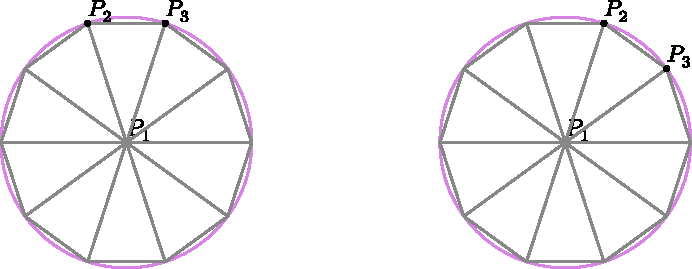
\includegraphics[width=0.4\textwidth]{res/figures/polosSphere.pdf}
    \caption{
        Ilustração da ligação dos vértices da primeira stack ao pólo norte, formando os triângulos
        iniciais da esfera e a seguinte iteração.
    }
\end{figure}

2. Ligação das stacks intermédias:
Para cada fatia horizontal da esfera, os vértices são ligados de forma a criar duas faces
triangulares por quadrilátero:
\[
T_1 = (P_1, P_3, P_4)
\]
\[
T_2 = (P_1, P_4, P_2)
\]

\begin{figure}[H]
    \centering
    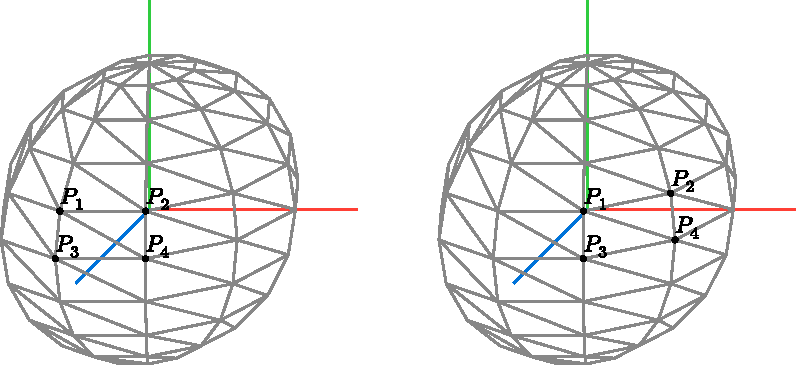
\includegraphics[width=0.4\textwidth]{res/figures/sphere.pdf}
    \caption{
        Triângulos de uma esfera gerada, e os pontos utilizados numa iteração do ciclo de geração
        de triângulos e na seguinte.
    }
\end{figure}

Este método assegura uma ligação contínua entre os pontos e evita a repetição de vértices
desnecessários.

3. Ligação ao pólo sul: O mesmo processo utilizado para o pólo norte é aplicado à stack
mais próxima do pólo sul, assim, garante que todas as fatias inferiores são corretamente ligadas ao
vértice final.
No entanto, a ordem dos vértices nos triângulos é invertida em comparação com o pólo norte.
Esta inversão garante que a normal de cada triângulo aponta para baixo, conforme ilustrado nos
círculos da primeira figura. No pólo norte, os vértices são ordenados no sentido anti-horário
(por exemplo, $P_1$, $P_3$, $P_2$), enquanto que no pólo sul, a ordem é invertida
($P_1$, $P_2$, $P_3$).

Este método proporciona uma representação eficiente e visualmente precisa, garante uma
boa distribuição das faces ao longo da sua superfície.

\subsection{Cilindro}

Para a construção do cilindro, utilizámos um sistema de coordenadas cilíndricas, onde a
posição de cada ponto é determinada pelo raio, pelo ângulo azimutal \( \phi \) e
pela altura \( y \).

A parametrização de um vértice sobre um cilindro de raio \( r \) e altura \( h \) pode ser definida
pelas seguintes equações:
\[
x = r \cos(\phi)
\]
\[
y = h
\]
\[
z = r \sin(\phi)
\]
onde:
\begin{itemize}
\item \( \phi \) é o ângulo azimutal, varia entre \( 0 \) e \( 2\pi \), que determina a
posição do ponto ao longo da circunferência da base.
\item \( y \) representa a altura, varia entre \( 0 \) (base inferior) e \( h \)
(base superior).
\end{itemize}

Este modelo matemático permite representar um cilindro tridimensionalmente. Para a sua implementação
computacional, discretizamos estes valores, onde é gerado um conjunto finito de pontos e faces que
aproximam à sua forma contínua.

\subsubsection{Geração dos Vértices}
Para discretizar a superfície do cilindro, o intervalo de \( \phi \) é dividido em slices
(segmentos verticais), enquanto a altura \( y \) é dividida em stacks (fatias horizontais).
Assim, os incrementos são calculados da seguinte forma:
\[
\Delta \phi = \frac{2\pi}{\text{slices}}, \quad \Delta y = \frac{h}{\text{stacks}}
\]

Os vértices são gerados da seguinte forma:

1. Criação da superfície lateral: Para cada stack ao longo da altura, iterámos
sobre os valores de \( \phi \), determinando a posição dos pontos na circunferência da secção
correspondente.

2. Criação dos vértices centrais das bases: Após gerar os pontos da superfície lateral,
adicionamos dois vértices centrais:
\begin{itemize}
\item O centro da base superior, localizado em \( (0, h, 0) \).
\item O centro da base inferior, localizado em \( (0, 0, 0) \).
\end{itemize}

\subsubsection{Construção das Faces}
Após a geração dos vértices, definimos as faces triangulares que compõem o cilindro. Esta etapa
é realizada em três partes:

1. Construção da superfície lateral:
Cada quadrilátero entre duas stacks sucessivas é dividido em duas faces triangulares:
\[
T_1 = (P_4, P_6, P_7)
\]
\[
T_2 = (P_4, P_7, P_5)
\]
Isto garante uma cobertura uniforme da superfície do cilindro.

\begin{figure}[H]
    \centering
    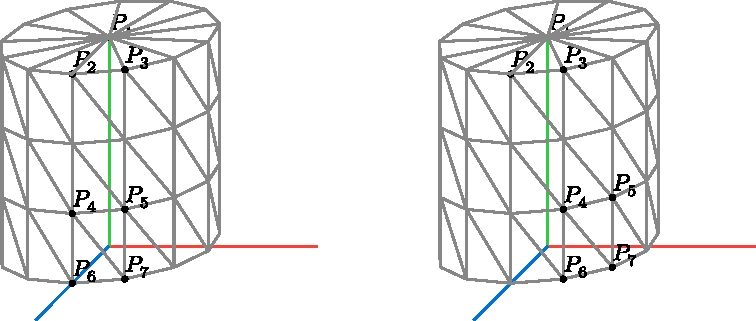
\includegraphics[width=0.4\textwidth]{res/figures/cylinder.pdf}
    \caption{
        Triângulos de uma esfera gerada, e os pontos utilizados numa iteração do ciclo de geração
        de triângulos e na seguinte.
    }
\end{figure}

2. Construção da base superior:
Cada ponto da última stack é ligado ao vértice central da base superior, de modo a formar
triângulos radiais:
\[
T = (P_1, P_2, P_3)
\]

3. Construção da base inferior:
O mesmo processo é repetido para a base inferior, o que garante o desenho correto da estrutura.

A ordem dos vértices cumpre a regra da orientação anti-horária, onde a correta
aplicação da técnica de face culling cumpre-se, que otimiza o processo de renderização
ao eliminar automaticamente as faces voltadas para trás.

Este método resulta numa representação eficiente e precisa do cilindro, mantendo uma boa
distribuição das faces sobre a sua superfície.

\subsection{Cone}

Para gerar a nuvem de pontos do cone, é necessário ter em atenção dois vértices especiais, o centro
da sua base e o vértice do seu topo, com as coordenadas abaixo:

$$
P_0 = (0, 0, 0)
\hspace{1cm}
P_n = (0, H, 0)
\hspace{1cm}
\text{, onde $H$ representa a altura do cone}
$$

\begin{figure}[H]
    \centering
    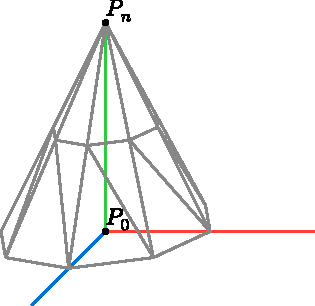
\includegraphics[width=0.35\textwidth]{res/figures/Cone1.pdf}
    \caption{Primeiro vértice ($P_0$) e último vértice ($P_n$) de um cone.}
\end{figure}

Os restantes vértices são todos obtidos do mesmo modo: para cada \emph{stack}, geram-se tantos
vértices quantos o número de \emph{slices}.

\begin{figure}[H]
    \centering
    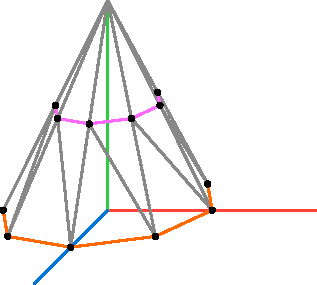
\includegraphics[width=0.4\textwidth]{res/figures/Cone2.pdf}
    \caption{
        Duas \emph{stacks} de um cone. Não são apresentados vértices ocultados pelas faces visíveis.
    }
\end{figure}

Para que as \emph{stacks} sejam equidistantes uma da outra, a distância entre \emph{stacks} será
o quociente entre a altura do cone e o número de \emph{stacks}. Por conseguinte, a coordenada $y$ da
$i$-ésima \emph{stack} será:

$$
y_i = \frac{H}{N_{stacks}} \times i
\hspace{1cm}
i \in \left \lbrace 0, 1, \ldots, N_{stacks} - 1 \right \rbrace
$$

Cada \emph{stack} no modelo será uma aproximação da secção transversal do cone por um plano
horizontal, ou seja uma circunferência. Na base do cone, o raio desta circunferência é o dado pelo
utilizador, $r$. Este raio tende para 0 à medida que se caminha para o vértice do topo do cone.
Logo, para a \emph{stack} $i$, o raio da circunferência a aproximar pode ser calculado por uma
interpolação linear:

$$
r_i = \frac{H - y_i}{H}\times r
\hspace{1cm}
i \in \left \lbrace 0, 1, \ldots, N_{stacks} - 1 \right \rbrace
$$

Dentro de cada $\emph{slice}$, as coordenadas $x$ e $z$ de cada ponto são determinadas de acordo
com a equação trigonométrica de uma circunferência:

$$
x = r_i \cos(\theta)
\hspace{1cm}
z = r_i \sin(\theta)
\hspace{1cm}
\theta \in \left [ 0, 2 \pi \right [
$$

Para se obterem tantos pontos quantas \emph{slices}, e para que estes estejam uniformemente
distribuídos pelo perímetro da circunferência, o ângulo $\theta$ é sempre incrementado em
$\frac{2 \pi}{N_{slices}}$ até o perímetro da circunferência ter sido coberto, dando origem à
seguinte equação de geração de pontos:

$$
x = r_i \cos \left ( \frac{2 \pi}{N_{slices}} \times j \right )
\hspace{1cm}
z = r_i \sin \left ( \frac{2 \pi}{N_{slices}} \times j \right )
\hspace{1cm}
j \in \left \lbrace 0, 1, \ldots, N_{slices} - 1 \right \rbrace
$$

Depois de estar criada a nuvem de pontos, constroem-se, em primeiro lugar, as faces triangulares da
base do cone. Para cada \emph{slice}, gera-se uma face, que tem  como vértices a origem ($P_0$), um
vértice da base ($P_1$), e o vértice da \emph{slice} seguinte ($P_2$), como mostra a figura abaixo:

\begin{figure}[H]
    \centering
    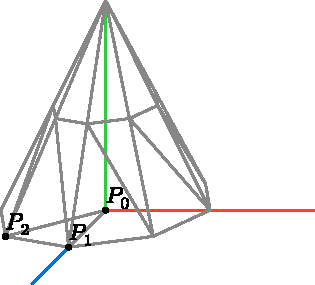
\includegraphics[width=0.4\textwidth]{res/figures/Cone3.pdf}
    \caption{
        \onehalfspacing
        Primeira iteração da construção das faces da base de um cone (com 8 \emph{slices} e 2
        \emph{stacks}).
    }
\end{figure}

Para que a normal desta face esteja voltada para fora do cone, ou seja, para baixo, os vértices do
triângulo são ordenados do seguinte modo, lembrando que esta ordem também se aplica aos restantes
vértices da base:

$$
T = (P_0, P_1, P_2)
$$

De seguida, constroem-se as faces laterais do cone, com exceção das da última \emph{stack} (a de
maior ordenada). É construído um quadrilátero (dois triângulos) por cada \emph{slice} na
\emph{stack}, utilizando um vértice da \emph{stack} ($P_1$), o seu adjacente seguinte na
\emph{stack} ($P_2$), e os dois pontos correspondentes a estes vértices na \emph{stack} seguinte
($P_9$ e $P_{10}$). A figura abaixo mostra os vértices utilizados na primeira iteração deste
processo:

\begin{figure}[H]
    \centering
    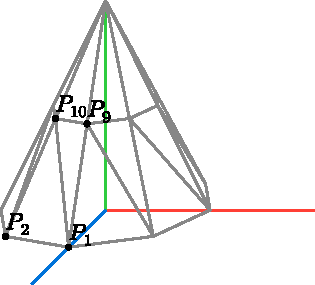
\includegraphics[width=0.4\textwidth]{res/figures/Cone4.pdf}
    \caption{
        \onehalfspacing
        Primeira iteração da construção das faces laterais de um cone (com 8 \emph{slices} e 2
        \emph{stacks}).
    }
\end{figure}

Para que os vetores normais destas faces apontem para fora do cone, utiliza-se a seguinte ordem para
os pontos dos triângulos, nesta e noutras iterações:

$$
T_1 = (P_1, P_9, P_{10})
\hspace{1cm}
T_2 = (P_1, P_{10}, P_2)
$$

Por último, constroem-se as faces da última \emph{stack}. Ao contrário do que acontece com as
restantes \emph{stacks}, já não se constroem quadriláteros, mas sim triângulos. Para cada
\emph{slice}, constrói-se um triângulo, formado pelo vértice do cone ($P_{17}$), por um vértice da
última \emph{stack} ($P_9$) e pelo vértice seguinte nessa \emph{stack} ($P_{10}$), como mostra a
figura abaixo:

\begin{figure}[H]
    \centering
    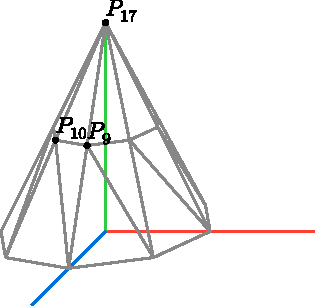
\includegraphics[width=0.4\textwidth]{res/figures/Cone5.pdf}
    \caption{
        \onehalfspacing
        Primeira iteração da construção das faces da última \emph{stack} de um cone (com 8
        \emph{slices} e 2 \emph{stacks}).
    }
\end{figure}

Para que estas faces sejam visíveis do exterior do cone, os seus vértices são ordenados do seguinte
modo:

$$
T = (P_9, P_{17}, P_{10})
$$

\subsection{Torus}

Matematicamente, as coordenadas de um ponto do \emph{torus} são definidas do seguinte modo
\cite{torus}:

$$
x = (-R + r \cos \phi) \cos \theta
\hspace{1cm}
y = r \sin \phi
\hspace{1cm}
z = (-R + r \cos \phi) \sin \theta
$$

$R$ e $r$ são os parâmetros dados para a geração do \emph{torus}, os raios maior e menor,
respetivamente. Os ângulos $\theta$ e $\phi$ variam ambos no intervalo $[0, 2\pi]$.

O ângulo $\theta$ define a rotação do ponto em torno do eixo central do torus, percorrendo o
círculo principal de raio $R$. Assim, ao variar $\theta$, o ponto desloca-se ao longo do anel do
torus, mantendo-se sempre na mesma posição relativa dentro do tubo. Já o ângulo $\phi$ determina a
posição do ponto dentro da secção transversal do tubo, que tem raio $r$. Ao variar $\phi$, o ponto
descreve um movimento circular dentro do tubo, movendo-se ao longo da circunferência menor do torus.

Para gerar uma nuvem de pontos uniformemente distribuídos, dividem-se os ângulos em fatias
($slices$) e segmentos ($stacks$), utilizando:

$$
\theta_i = i \cdot \frac{2\pi}{slices}, \quad i \in \{0, 1, \ldots, slices\}
$$

$$
\phi_j = j \cdot \frac{2\pi}{stacks}, \quad j \in \{0, 1, \ldots, stacks\}
$$

Assim, o torus é gerado iterando sobre os valores inteiros possíveis de $i$ e $j$, incrementando
primeiro $j$ e só depois $i$, o que dá origem à nuvem de pontos desejada.

Após a geração dos vértices, estes são agrupados nos triângulos que compõem a superfície do torus.
Para isso, considera-se um vértice de referência, como $P_1$, juntamente com o vértice adjacente
na mesma fatia ($P_3$) e os dois vértices correspondentes na fila seguinte da fatia ($P_2$ e
$P_4$).
Este processo repete-se para todos os vértices aplicáveis, garantindo que cada célula quadrangular
seja subdividida em dois triângulos. A figura seguinte ilustra esse processo, mostrando a estrutura
da nuvem e a organização dos triângulos resultantes.

\begin{figure}[H]
    \centering
    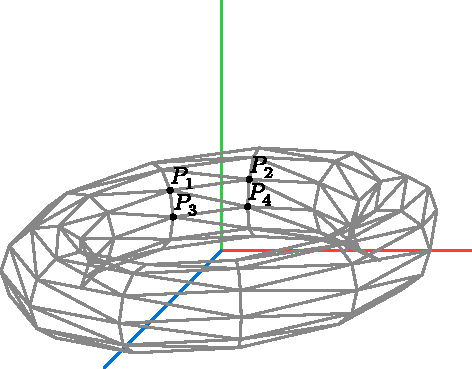
\includegraphics[width=0.4\textwidth]{res/figures/TorusTriangle.pdf}
    \caption{Triângulos de um torus gerado. As faces ocultas não são apresentadas.}
\end{figure}

Pretende-se que os triângulos do \emph{torus} estejam voltados para fora, pelo que os seus vértices
devem estar ordenados na ordem contrária à dos ponteiros do relógio. Para os quatro pontos
apresentados acima, os triângulos gerados são os seguintes:

$$
T_1 = (P_1, P_2, P_3)
\hspace{1cm}
T_2 = (P_2, P_4, P_3).
$$

O \emph{torus} é a única superfície côncava gerada, o que trás problemas relativos à orientação das
suas normais. As normais de todas as faces apontam para "fora"{} do \emph{torus}, ou seja, as das
faces interiores ("do buraco"{}) apontam para o centro do \emph{torus}, e as das faces exteriores
apontam no sentido contrário.

Idealmente, a parte interna do \emph{torus} não deveria ser visível quando este é observado de fora,
pois a própria geometria bloquearia essa visão. No entanto, como apenas os contornos das faces são
desenhados, e a direção das normais é o único critério utilizado de momento para determinar se uma
face é ou não desenhada, pode ocorrer um efeito onde a parte interna do \emph{torus} é visível, como
mostra a figura abaixo. Esse fenómeno acontece porque as normais da parte interna apontam para a
câmara, tal como as normais das faces que a deveriam cobrir.

\textbf{\color{red} TODO - figura com a cena do torus}

Este problema será mitigado na fase 4 do trabalho, onde a superfície dos polígonos será preenchida
por completo, e as faces internas do \emph{torus} serão cobertas pelas faces externas.

\section{\emph{Engine}}

\subsection{Cena (\texttt{Scene})}

A classe \texttt{Scene} assume um papel fulcral na \texttt{engine}, pois é responsável por
interpretar ficheiros XML com os conteúdos que devem ser renderizados. Para a sua análise sintática
destes ficheiros, a biblioteca \texttt{TinyXML2} \cite{tinyxml2} é utilizada. Segue um exemplo de
uma cena em formato XML:

% TODO - adjust listing style and syntax highlighting after merging

\begin{lstlisting}

<world>
    <window width="512" height="512" />
    <camera>
        <position x="3" y="2" z="1" />
        <lookAt x="0" y="0" z="0" />
        <up x="0" y="1" z="0" />
        <projection fov="60" near="1" far="1000" />
    </camera>
    <group>
        <models>
            <model file="../models/box.3d" />
        </models>
    </group>
</world>
\end{lstlisting}

O processo de análise inicia-se com a leitura do elemento raiz, \texttt{<world>}, que contêm todos
os elementos de configuração. A \texttt{Scene} começa por extrair as dimensões da janela a partir do
elemento \texttt{<window>} e as propriedades da câmara a partir do elemento \texttt{<camera>}.
Depois, prossegue à leitura dos objetos presentes na cena. Os elementos \texttt{<group>} podem
conter outros elementos \texttt{<group>}, ou então elementos \texttt{<model>}, que especificam os
modelos 3D a serem carregados e renderizados. Nesta primeira fase, por simplicidade, esta estrutura
hierárquica é linearizada durante o carregamento de uma cena (a \texttt{engine} armazena um
\texttt{std::vector} de modelos), mas isto é algo que terá de ser mudado para suportar as
transformações geométricas da próxima fase.

O leitor de cenas procura evitar o carregamento do mesmo modelo mais do que uma vez. Com recurso a
um dicionário (\texttt{std::unordered\_map}), são armazenados os modelos já carregados. Quando um
elemento \texttt{<model>} é encontrado, caso este refira um ficheiro \texttt{.3d} carregado
anteriormente, ele é reutilizado; caso contrário, um novo modelo é carregado e armazenado no
dicionário.

A classe \texttt{Scene} também é responsável por desenhar os conteúdos de uma cena. Para o fazer,
começa por configurar a matriz da câmara no \emph{shader} de vértices, e itera por todas as
entidades, desenhando cada uma.

\subsection{Entidade (\texttt{Entity})}

A classe \texttt{Entity} representa um objeto 3D individual na cena, combinando um modelo
(\texttt{Model}) com outra informação relevante como, por exemplo, a sua cor. Esta classe é também
responsável por renderizar cada objeto corretamente, transformando o seu modelo de acordo com os
atributos definidos.

Uma otimização feita à \texttt{Entity} é o uso de um \texttt{std::shared\_ptr<Model>} para
referenciar o modelo associado a cada objeto. Este apontador inteligente permite a partilha do mesmo
modelo por várias entidades que o usem, reduzindo o consumo de memória da GPU. Ademais, o uso de
contagem de referências permite a libertação automática de memória, seguindo os princípios RAII de
C++.

\subsection{Criação da janela}

Para a criação da janela, a biblioteca GLFW foi utilizada \cite{glfw}, escolhida principalmente pela
sua API moderna. Ao contrário do GLUT \cite{glut}, utilizado nas aulas práticas da UC, a API do GLFW
não obriga a guardar o estado da aplicação em variáveis globais para que os métodos associados à
janela lhe possam aceder. Isto possibilita a criação de abstrações RAII em torno da janela criada, o
que por sua vez permite a utilização das várias funcionalidades de C++ para gestão automática de
memória. Ademais, a API do GFLW também permite um maior controlo sobre o ciclo de resposta a eventos
e renderização.

Já na primeira fase do projeto, optou-se por utilizar uma versão do OpenGL mais atual do que a que é
utilizada nas aulas práticas, o \emph{core profile} do OpenGL 4.6. Apesar do seu uso exigir um maior
esforço na primeira fase, com a utilização obrigatória de VBOs e de \emph{shaders}, esta versão
suporta mais funcionalidades do que as versões anteriores, permite obter um melhor desempenho, e é
suportada por depuradores como RenderDoc \cite{renderdoc}. Para utilizar esta versão de OpenGL, um
\emph{loader} é necessário, e o GLAD \cite{glad} foi escolhido devido ao seu elevado grau de
personalização.

\subsection{Comportamento da \emph{engine}}

O primeiro passo na execução da \emph{engine} é a criação da janela e do seu contexto OpenGL. Este é
necessário para os passos seguintes: a leitura da cena, onde é necessário criar VBOs para os
modelos 3D, a instanciação dos eixos do sistema de coordenadas, também suportados por VBOs, e a
criação dos \emph{shaders} de vértices e de fragmentos. Uma vez que os VBOs e os \emph{shaders} não
são um objetivo da primeira fase deste trabalho, o seu funcionamento só será descrito em detalhe num
relatório futuro.

Estando inicializada a \emph{engine}, segue-se um ciclo em que a janela reage a eventos e desenha os
seus conteúdos. Neste ciclo, são suportados os eventos de passagem de tempo, necessidade de
atualizar os conteúdos da janela, e redimensionamento da janela. Para se subscrever a um evento,
basta sobrescrever o seu método correspondente na classe \texttt{Window}:

\begin{lstlisting}

virtual void onUpdate(float time, float timeElapsed) = 0;
virtual void onRender() = 0;
virtual void onResize(int width, int height) = 0;
\end{lstlisting}

De momento, apenas os métodos \texttt{onRender} e \texttt{onResize} são utilizados. Nestes,
desenham-se os conteúdos da janela e atualiza-se a matriz de projeção da câmara, respetivamente. Em
relação ao processo de renderização, este consiste no envio da matriz da câmara para o \emph{shader}
de vértices, na renderização dos eixos usando \texttt{glDrawArrays}, e na iteração por todos os
objetos da cena, usando \texttt{glDrawElements} para desenhar cada um. No futuro, serão adicionados
métodos de resposta a eventos de \emph{input} do utilizador, que o permitirão executar ações como,
por exemplo, mover a câmara.

\subsection{Câmara}

A câmara é responsável por definir a perspetiva e o enquadramento da cena 3D. A sua configuração
segue um modelo de câmara em primeira pessoa, com a posição, orientação e projeção definidas a
partir do ficheiro XML da cena.

A posição da câmara é representada pelo vetor \texttt{position}, que define a sua localização no
espaço tridimensional. A direção para onde a câmara está orientada é determinada pelo vetor
\texttt{lookAt}, um ponto no espaço para onde a lente da câmara aponta. O vetor \texttt{up}
especifica a orientação vertical da câmara, garantindo a sua correta rotação no espaço. Estes três
vetores são utilizados para calcular a matriz de visualização.

Uma vez que este projeto usa \emph{shaders}, não é possível utilizar a função \texttt{gluLookAt}
\cite{gluLookAt}, usada nas aulas práticas para o cálculo da matriz de visualização. No entanto,
como utilizamos a biblioteca \texttt{glm} \cite{glm}, é usada a função equivalente
\texttt{glm::lookAt}, que devolve uma matriz que pode ser passada ao \emph{shader} de vértices.

A projeção da câmara é controlada pelo campo de visão (\emph{Field of View} -- FOV) e pelos planos
de recorte próximo e distante (\texttt{near} e \texttt{far}). O FOV define o ângulo de abertura da
câmara, influenciando a sensação de profundidade da cena, enquanto os planos de recorte estabelecem
os limites mínimo e máximo da região visível. A matriz de projeção é calculada com a função
\texttt{glm::perspective}, que utiliza o $FOV$, o \emph{aspect ratio} da janela, e os planos de
recorte para definir a forma como os objetos são projetados no espaço 3D.

A matriz final da câmara resulta da multiplicação da matriz de projeção pela matriz de visualização,
e é atualizada sempre que a janela é redimensionada. É utilizada para transformar todos os objetos
da cena, garantindo um enquadramento adequado dos mesmos e a renderização correta da cena.

De momento, a \texttt{engine} não suporta que o utilizador controle a posição da câmara
dinamicamente, movendo-a após a leitura do ficheiro XML. No entanto, pretendemos implementar esta
funcionalidade na segunda fase do projeto.

\section{Resultados obtidos}

\textbf{\color{red} TODO - resultados}

\section{Conclusão e Trabalho Futuro}

\textbf{\color{red} TODO - conclusão}

\begingroup
\section{Bibliografia}
\renewcommand{\section}[2]{}

\begin{thebibliography}{9}
    \bibitem{tinyxml2}
        "TinyXML-2."{} GitHub. Mar. 2, 2025. [Online.] Available:
        \url{https://github.com/leethomason/tinyxml2}
    \bibitem{wavefront-obj}
        "Wavefront OBJ File Format Summary."{} FileFormat.Info. Accessed: Mar. 2, 2025. [Online.]
        Available: \url{https://www.fileformat.info/format/wavefrontobj/egff.htm}
    \bibitem{esfera}
        "OpenGL Sphere."{} Songho CA. Accessed: Mar. 1, 2025. [Online.] Available:
        \url{https://www.songho.ca/opengl/gl_sphere.html}
    \bibitem{cilindro}
        "OpenGL Cylinder, Prism \& Pipe."{} Songho CA. Accessed: Mar. 1, 2025. [Online.] Available:
        \url{https://www.songho.ca/opengl/gl_cylinder.html}
    \bibitem{torus}
        "Torus."{} Wolfram MathWorld. Accessed: Mar. 1, 2025. [Online.] Available:
        \url{https://mathworld.wolfram.com/Torus.html}
    \bibitem{glfw}
        "An OpenGL library."{} GLFW. Accessed: Feb. 27, 2025. [Online.] Available:
        \url{https://www.glfw.org}
    \bibitem{glut}
        "About."{} The freeglut project. Accessed: Feb. 27, 2025. [Online.] Available:
        \url{https://freeglut.sourceforge.net/}
    \bibitem{gluLookAt}
        "gluLookAt."{} Khronos Registry. Accessed: Mar. 2, 2025. [Online.] Available:
        \url{https://registry.khronos.org/OpenGL-Refpages/gl2.1/xhtml/gluLookAt.xml}
    \bibitem{glm}
        "glm."{} GitHub. Accessed: Mar. 2, 2025. [Online.] Available:
        \url{https://github.com/g-truc/glm}
    \bibitem{exemplo}
        \href{https://youtu.be/dQw4w9WgXcQ}{Um item de exemplo na bibliografia}
    \bibitem{renderdoc}
        "RenderDoc."{} RenderDoc Accessed: Feb. 28, 2025. [Online.] Available:
        \url{https://renderdoc.org/}
    \bibitem{glad}
        "Glad - Multi-Language GL/GLES/EGL/GLX/WGL Loader-Generator based on the official specs."{}
        Feb. 28, 2025. [Online.] Available: \url{https://glad.dav1d.de/}
\end{thebibliography}
\endgroup

\end{document}
